\documentclass{beamer}
\usetheme{Stockton}
%\usetheme{Warsaw}
%\usetheme{Frankfurt}
%\usetheme{Berlin}
\usepackage[T1]{fontenc}
\usepackage[utf8]{inputenc}
\usepackage{lmodern}
\usepackage{comment}
\usepackage{blindtext}
\usepackage{verbatim}
\usepackage{setspace}
\usepackage{subcaption}
\title{Creating Presentations}
\author{D. Aravinthan}

\begin{document}

\begin{frame}
  \titlepage
\end{frame}
%%%%%%%%%%%%%%%%%%%%%%%%%%%%%%%%%%%%%%%%%%%%%%%%%%%%%%%%%%%%%%%%%%%%%%%%%%%%%%%%%%%%%%%%%%%%%%%%%%%%%%%%%%%%%%
\begin{frame}[fragile]
\frametitle{Including Graphics}
%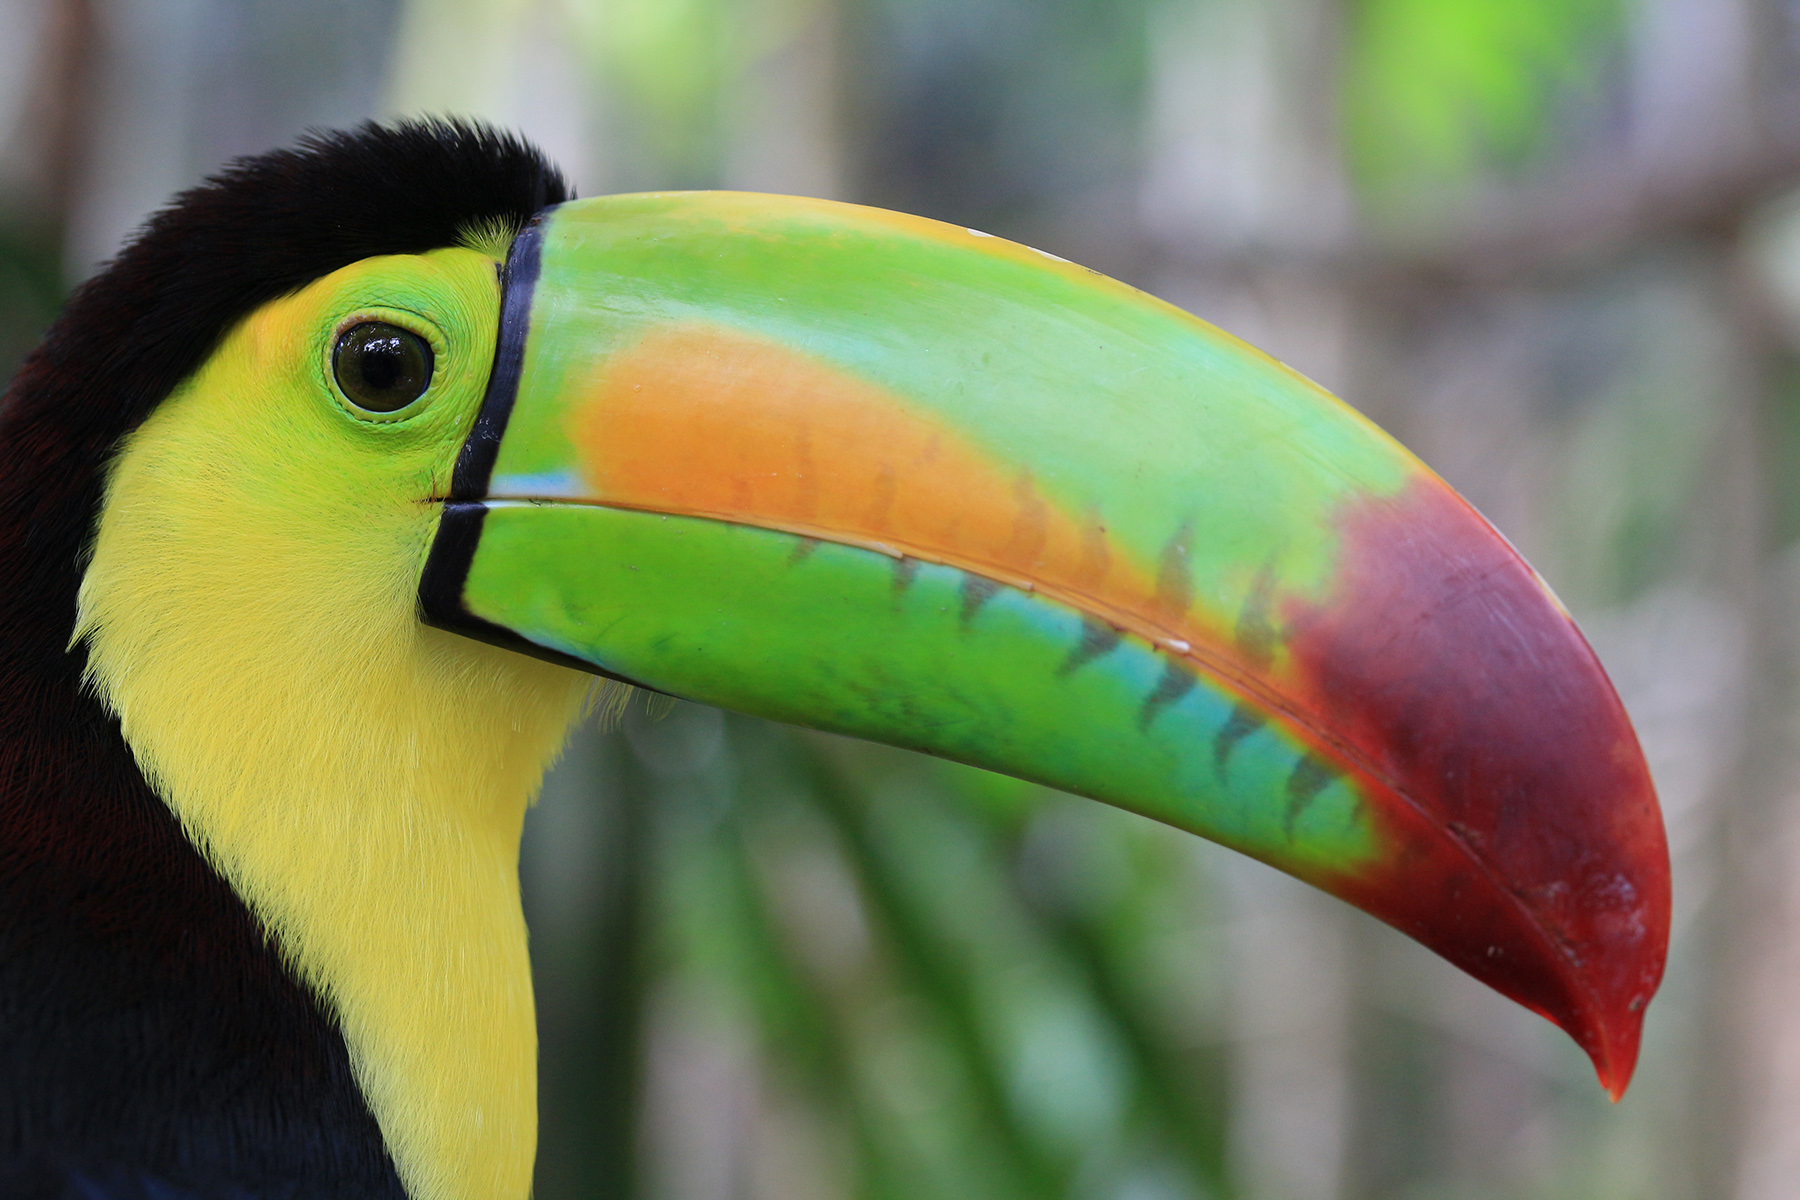
\includegraphics{sample1}
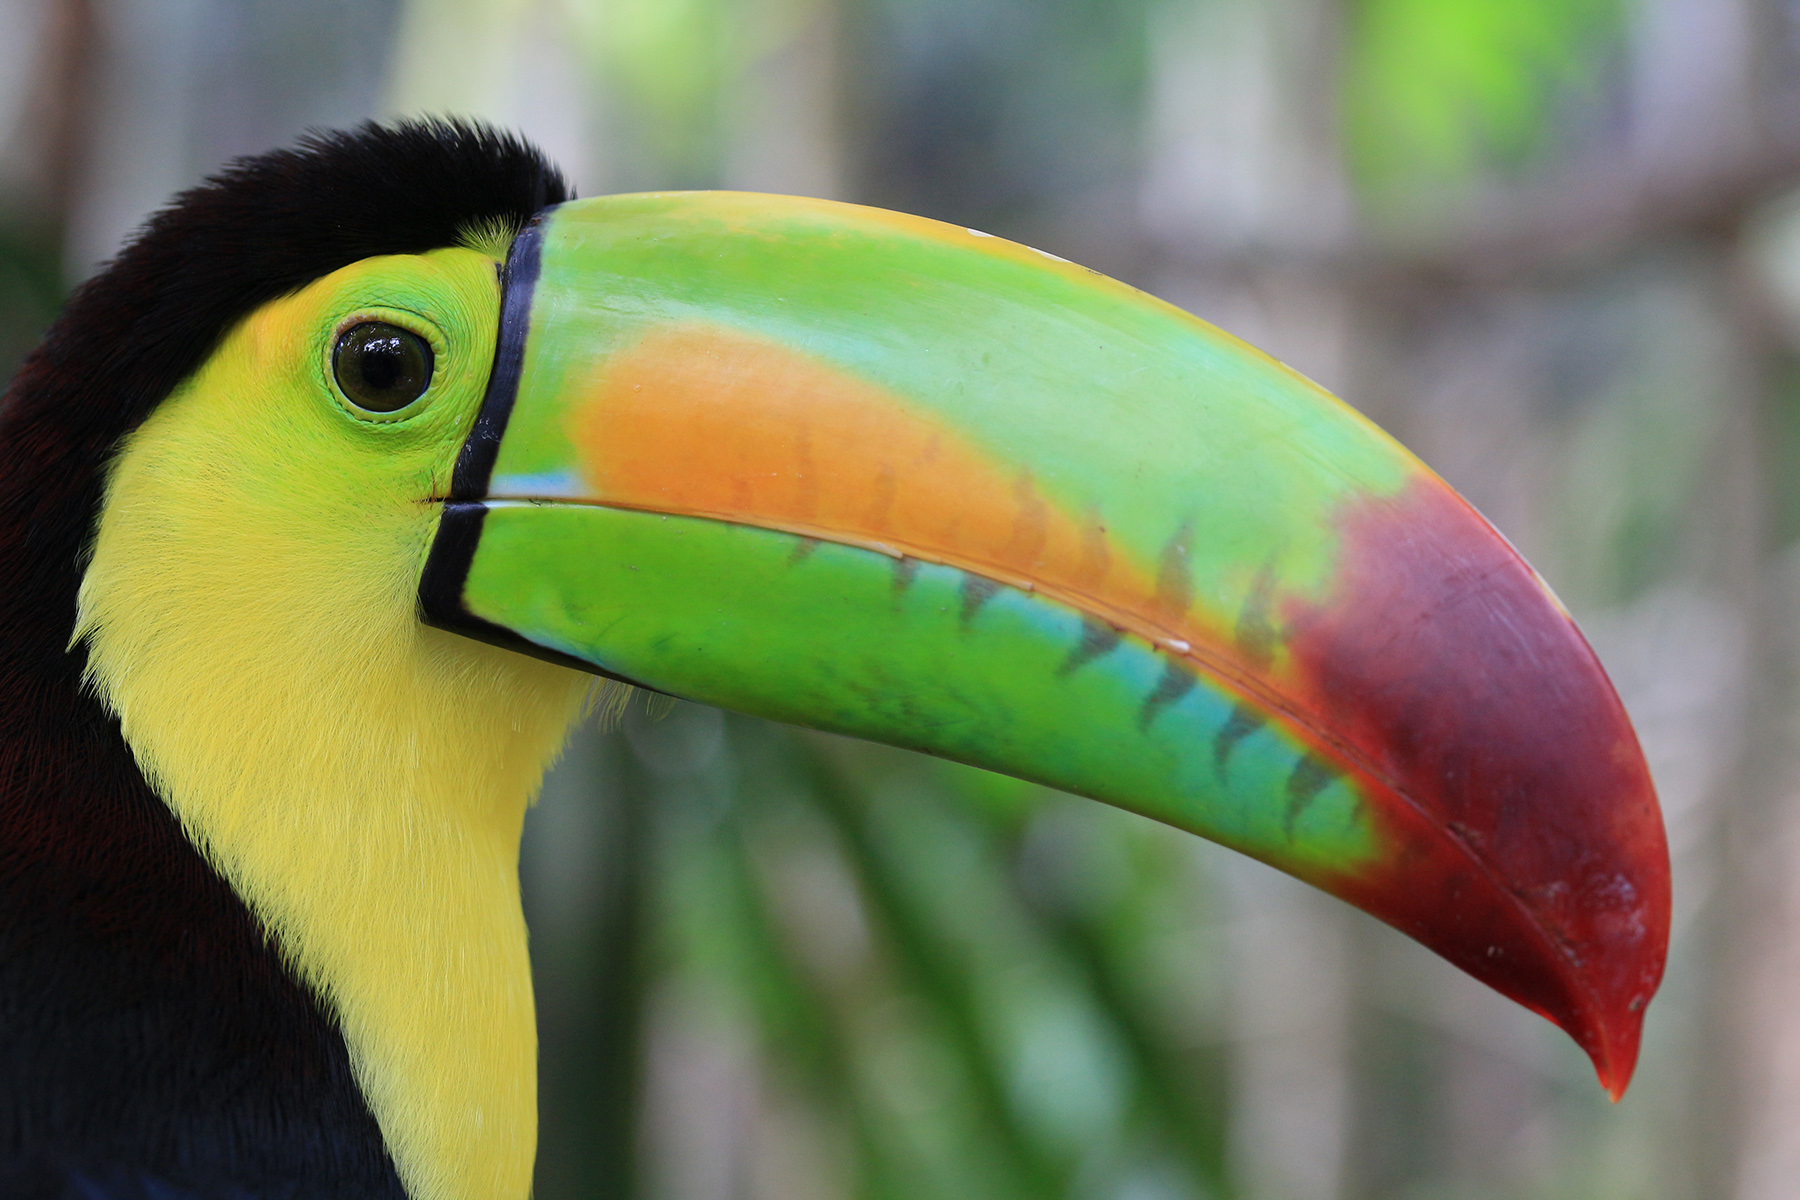
\includegraphics[scale=0.15]{sample1}
%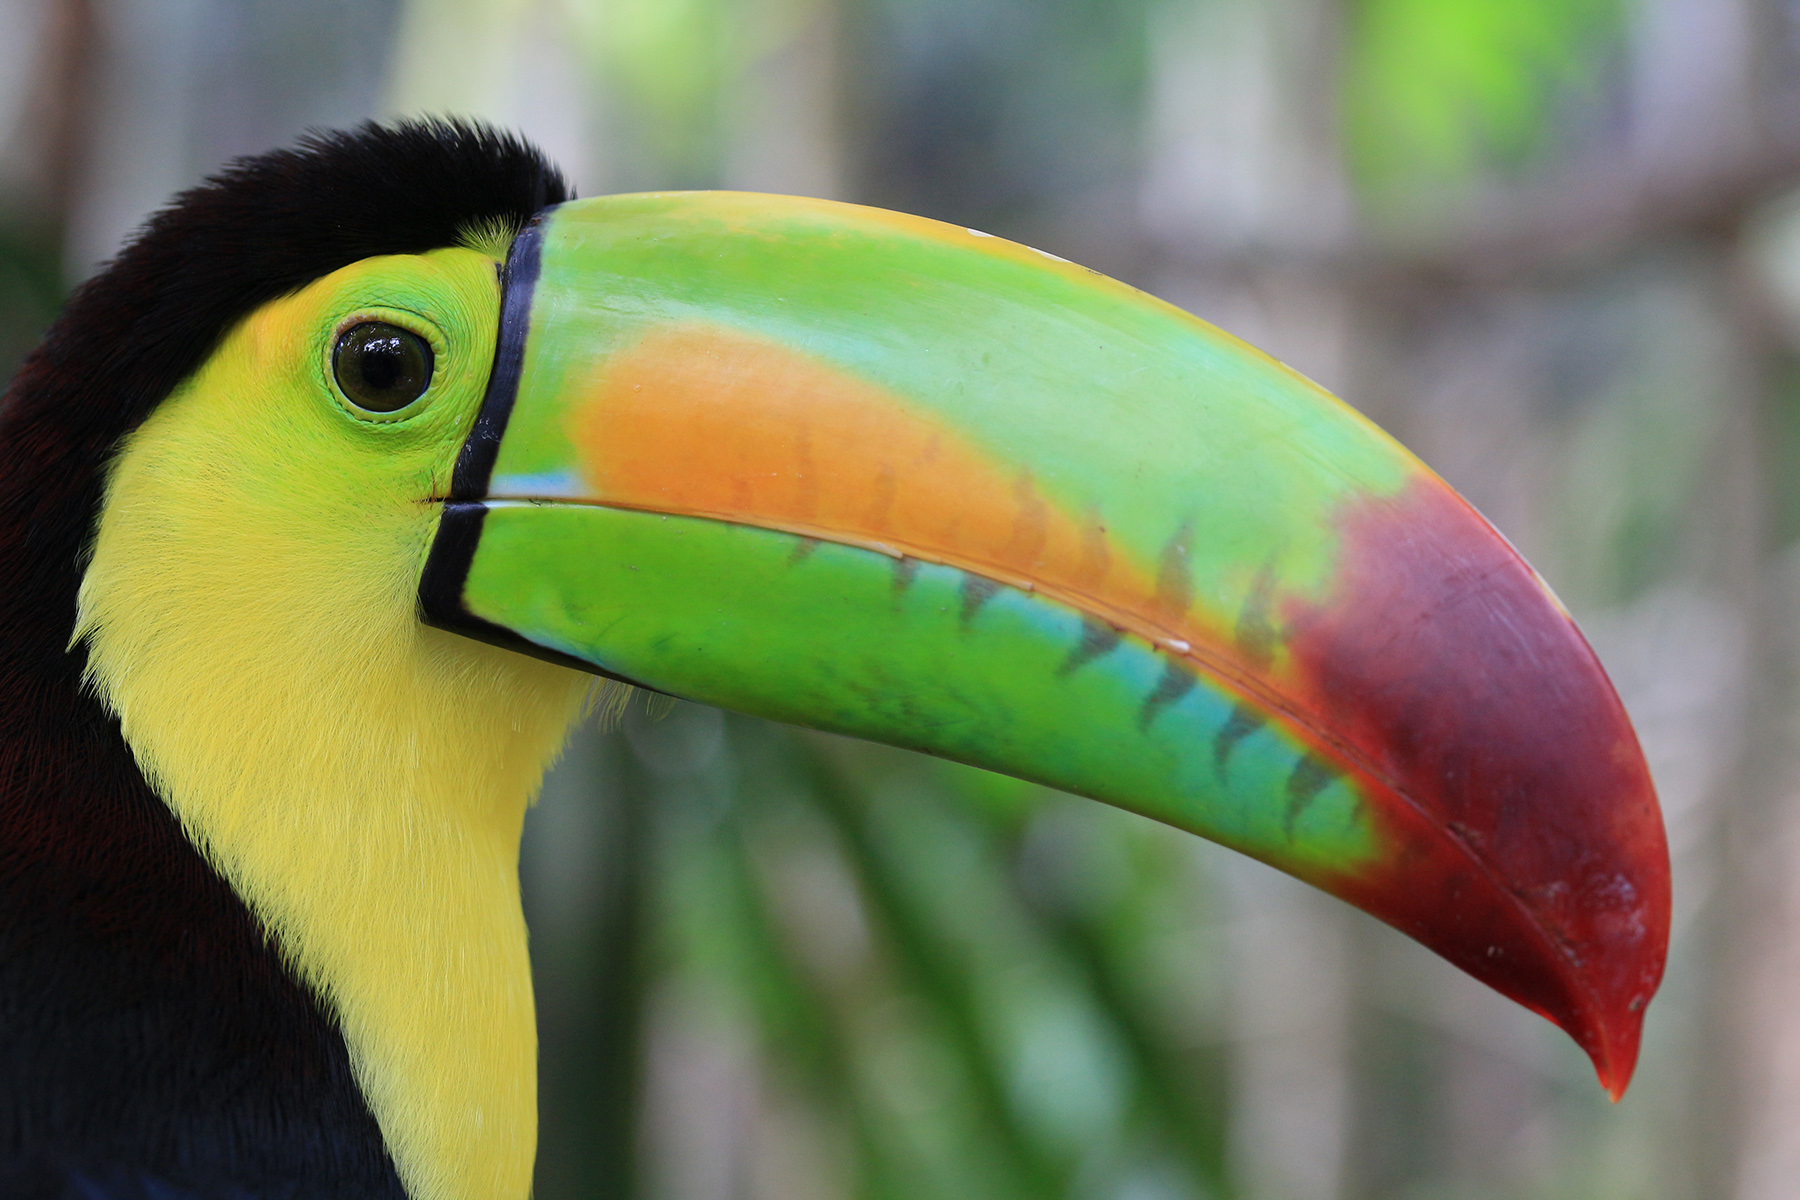
\includegraphics[height=1.5in]{sample1}
%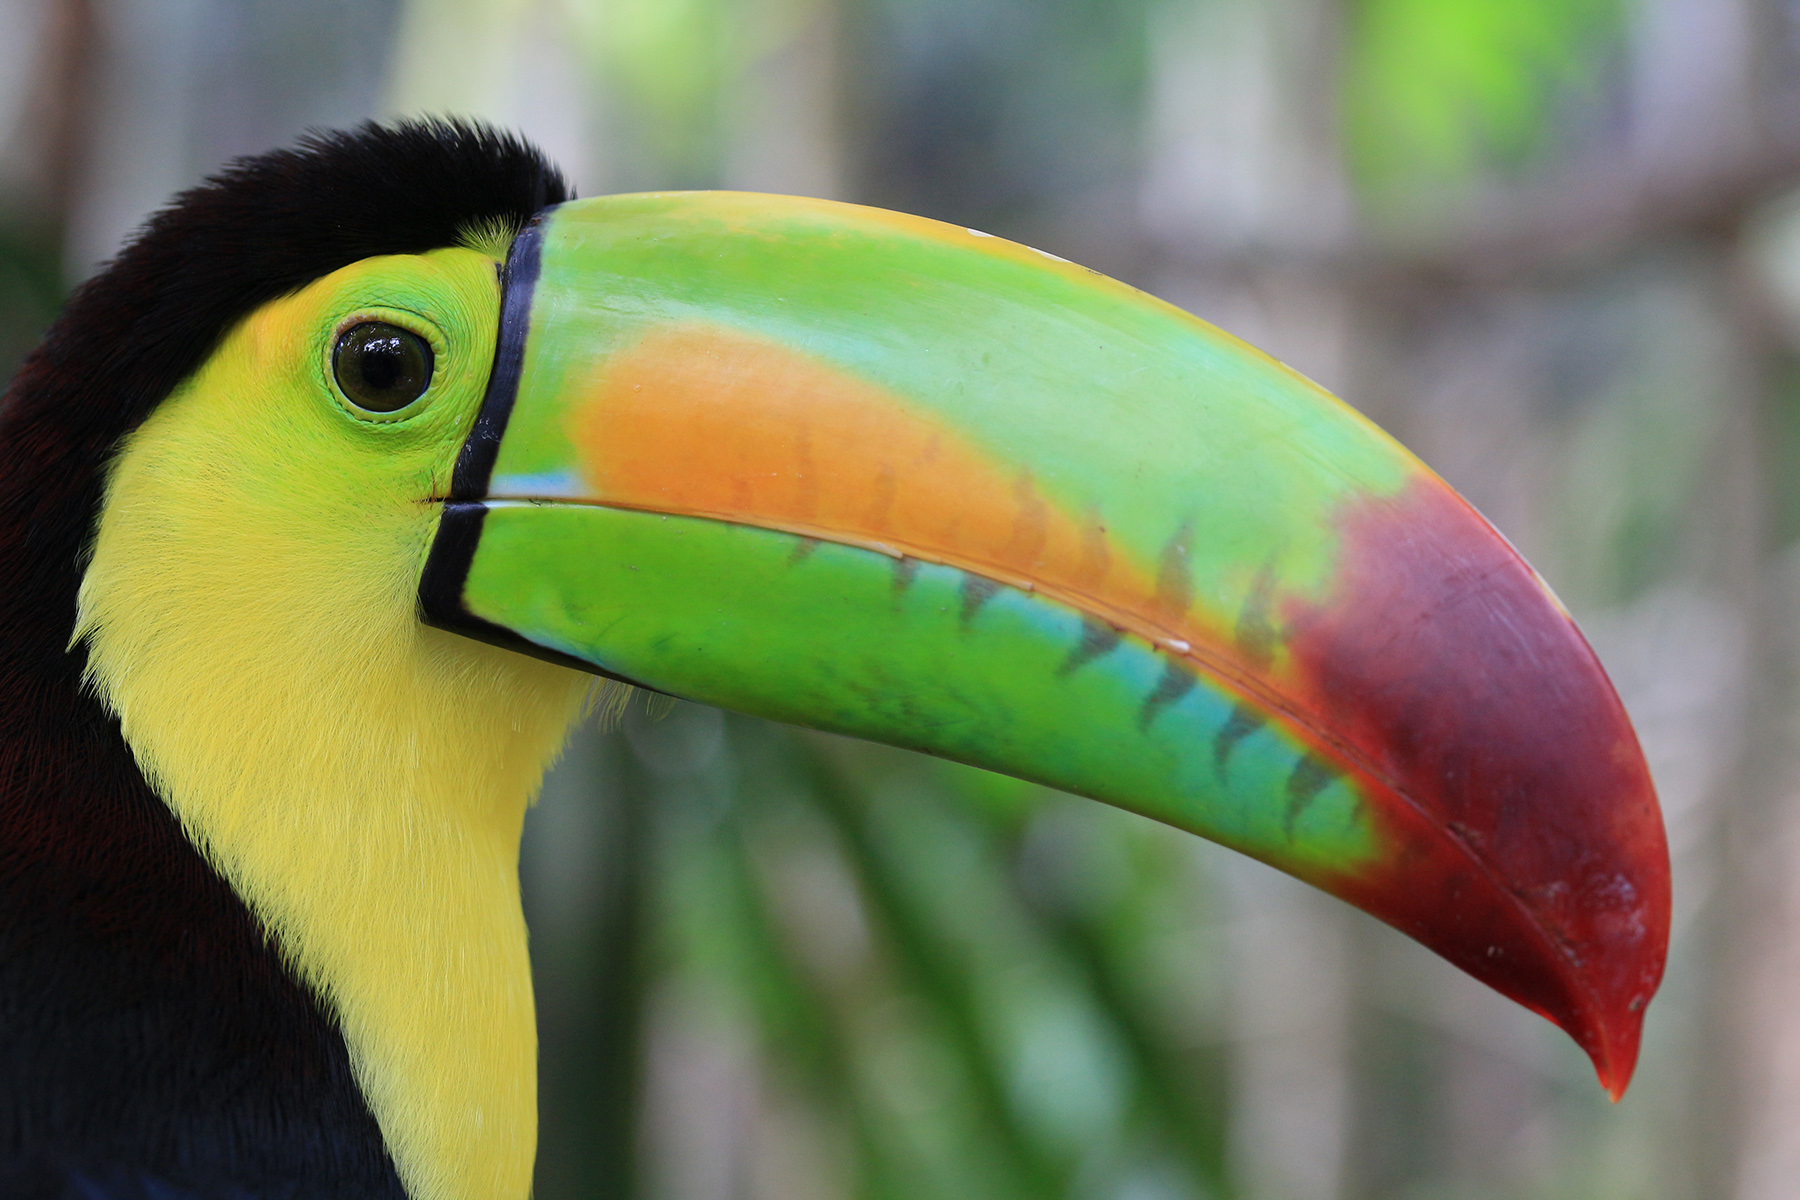
\includegraphics[height=7.5cm]{sample1}
%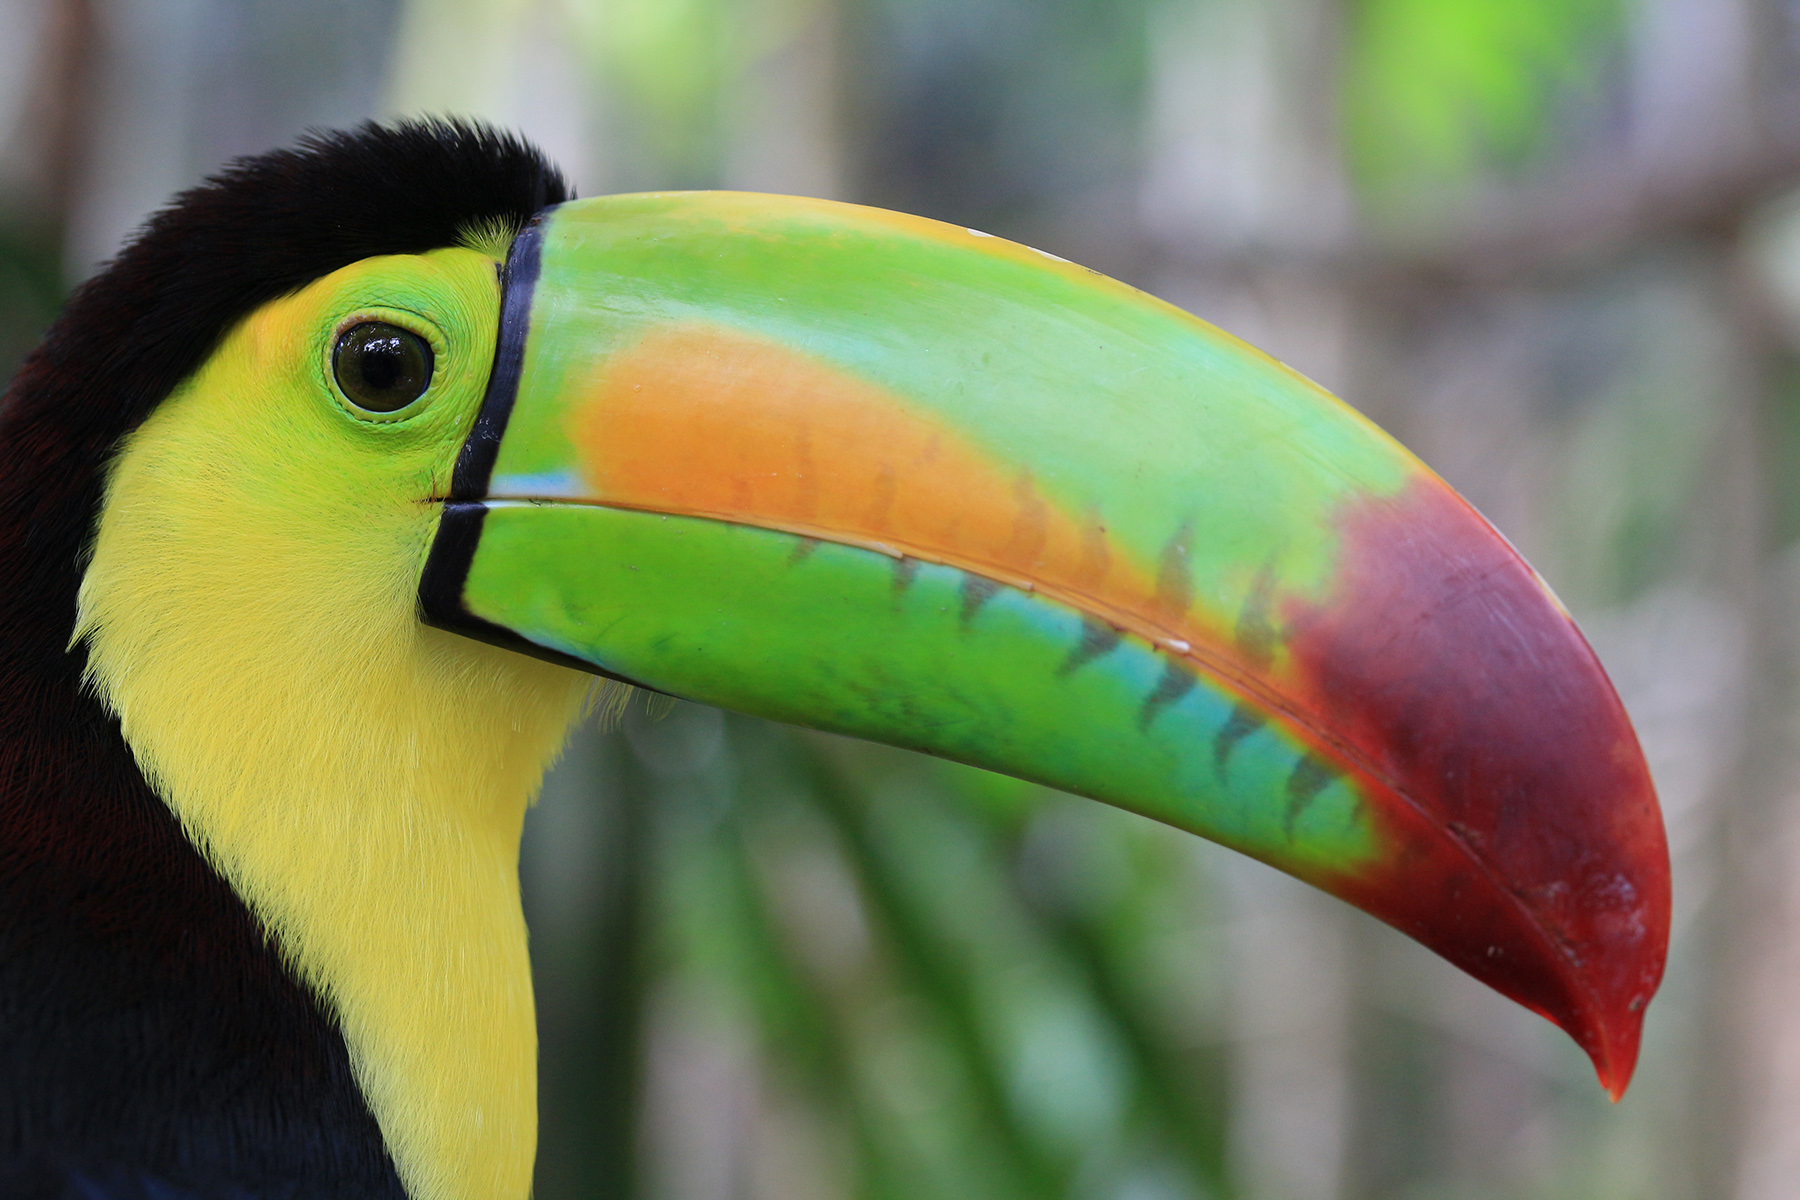
\includegraphics[width=7.5cm]{sample1}
%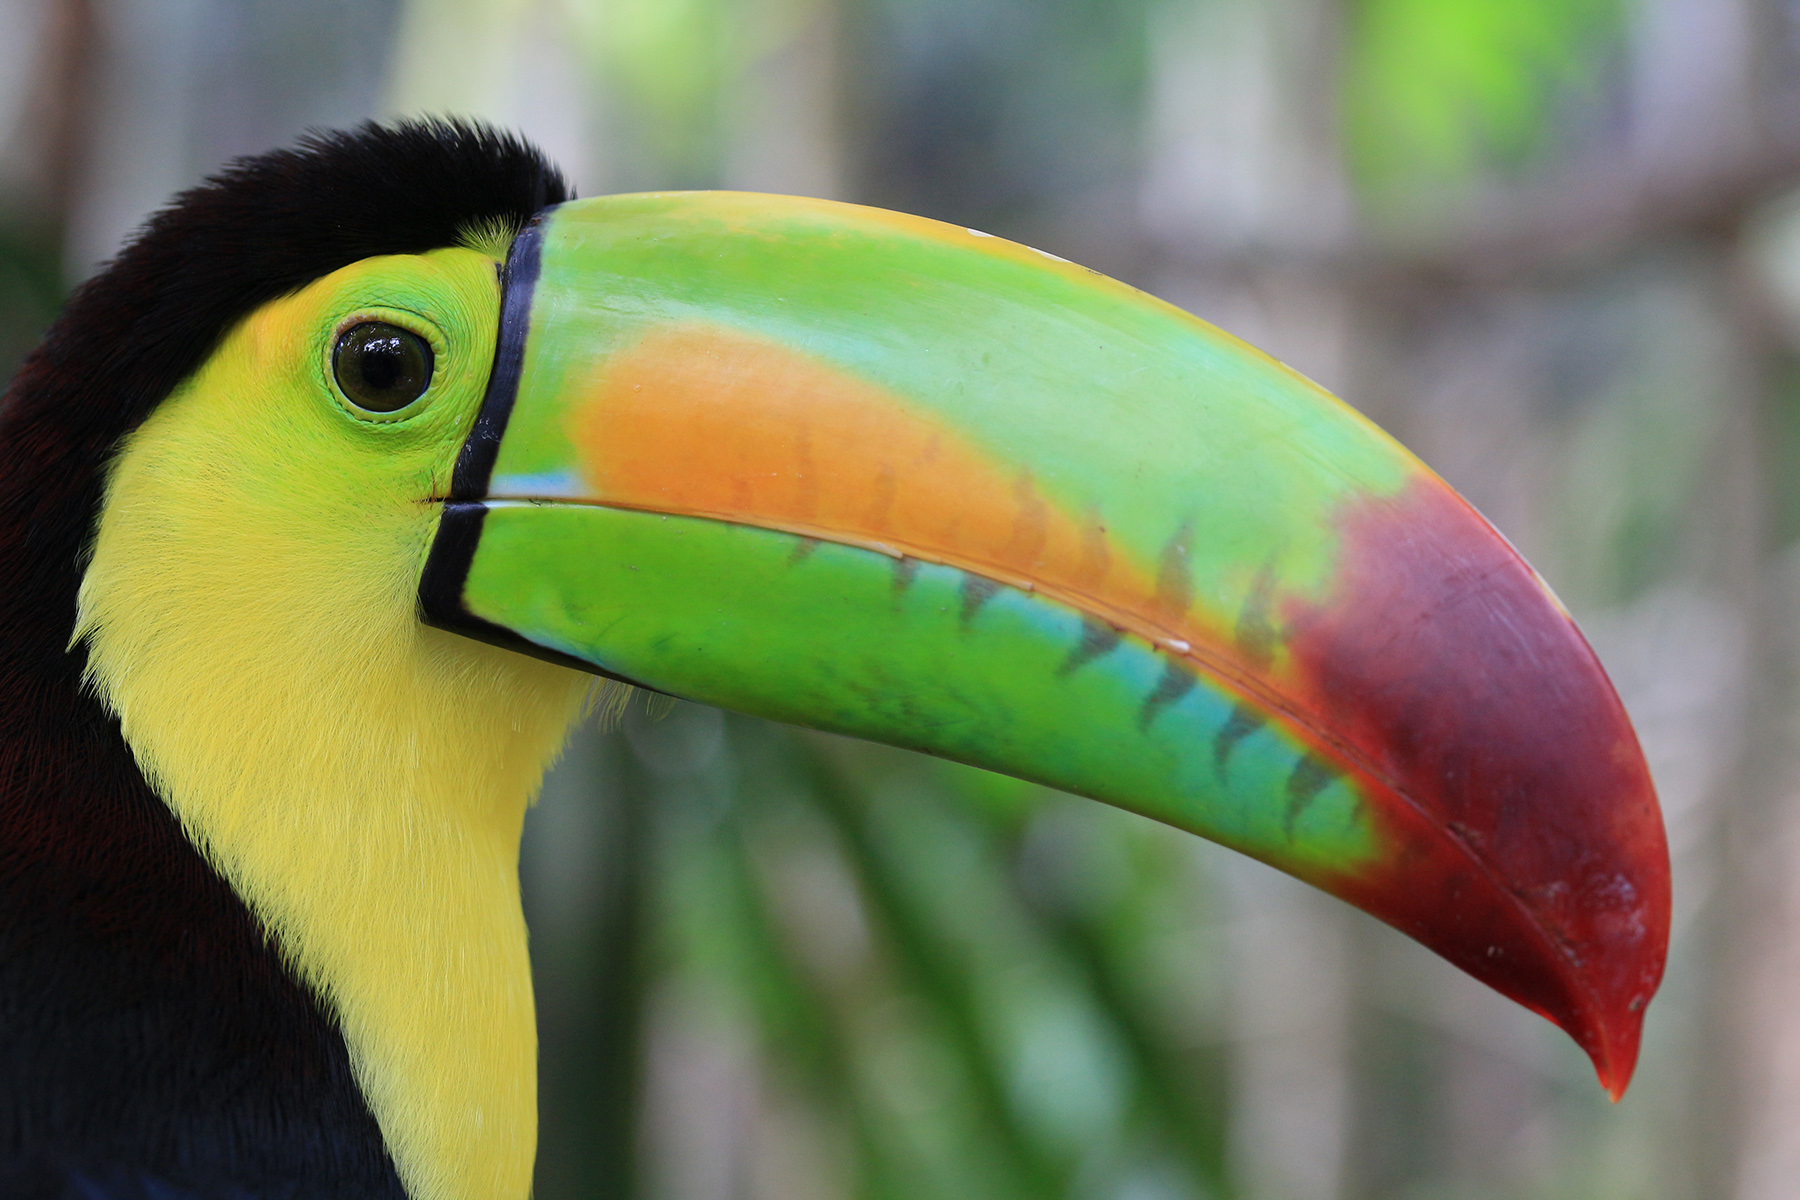
\includegraphics[height=2.5in,width=3.5in]{sample1}
%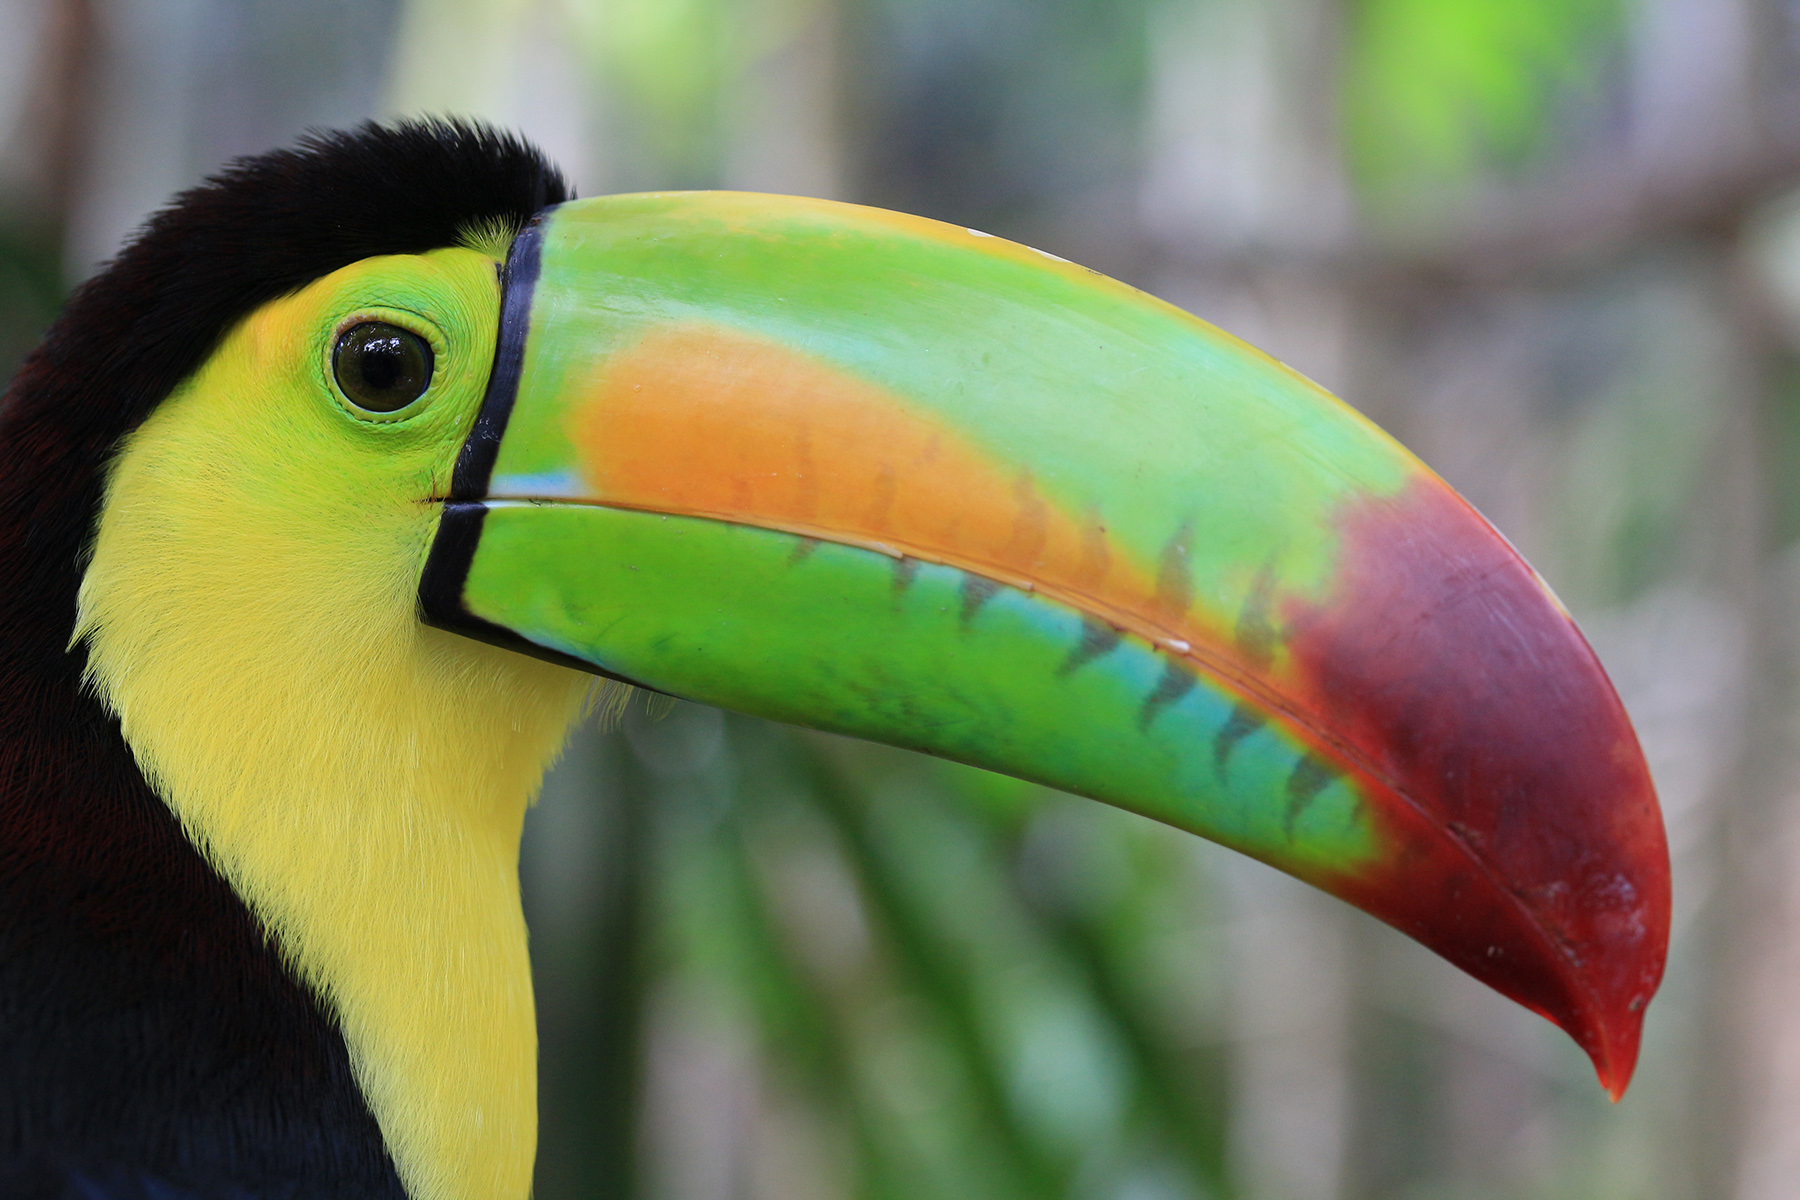
\includegraphics[height=2.in,width=3.in,angle=90]{sample1}
\begin{comment}
\begin{figure}
  \begin{center}
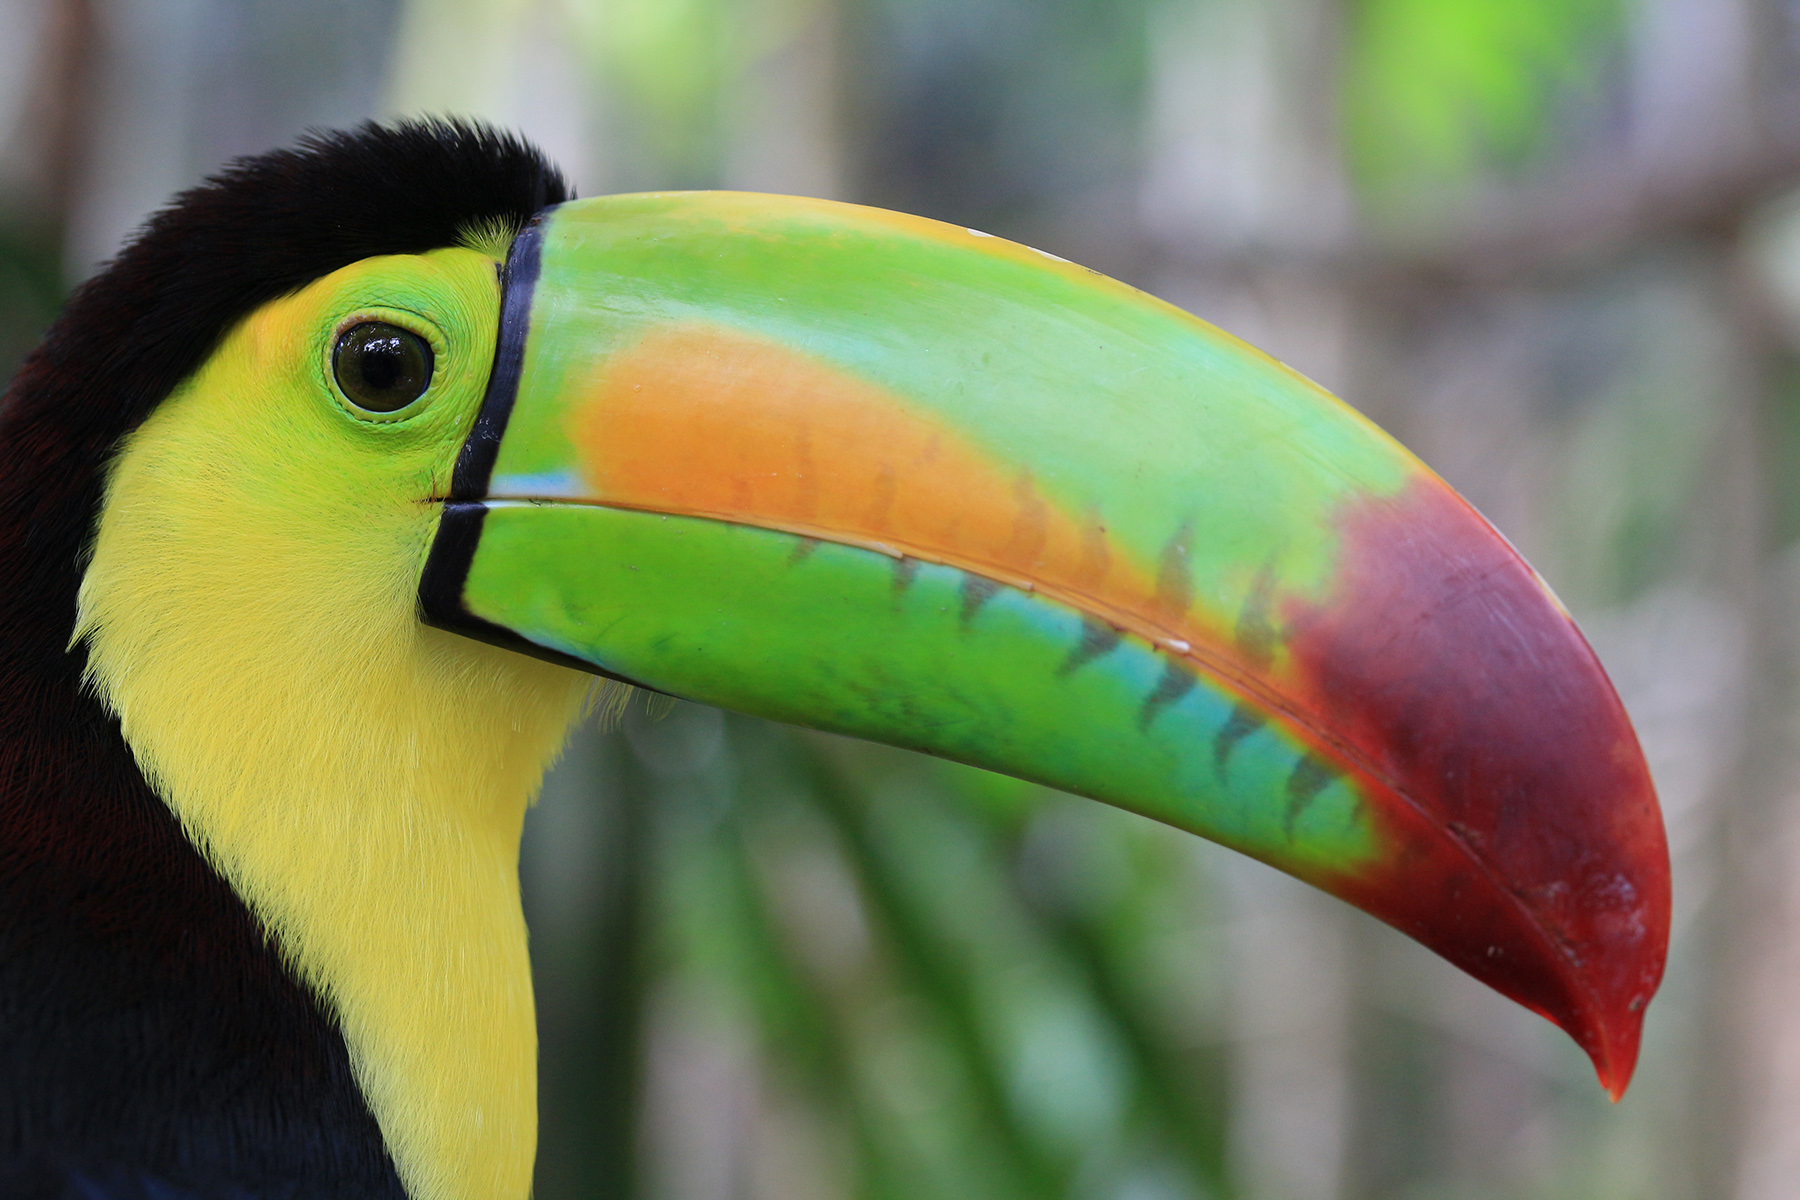
\includegraphics[height=2.in,width=3.in]{sample1}
    \caption{Figure with caption}
    \label{fig:}
  \end{center}
\end{figure}
%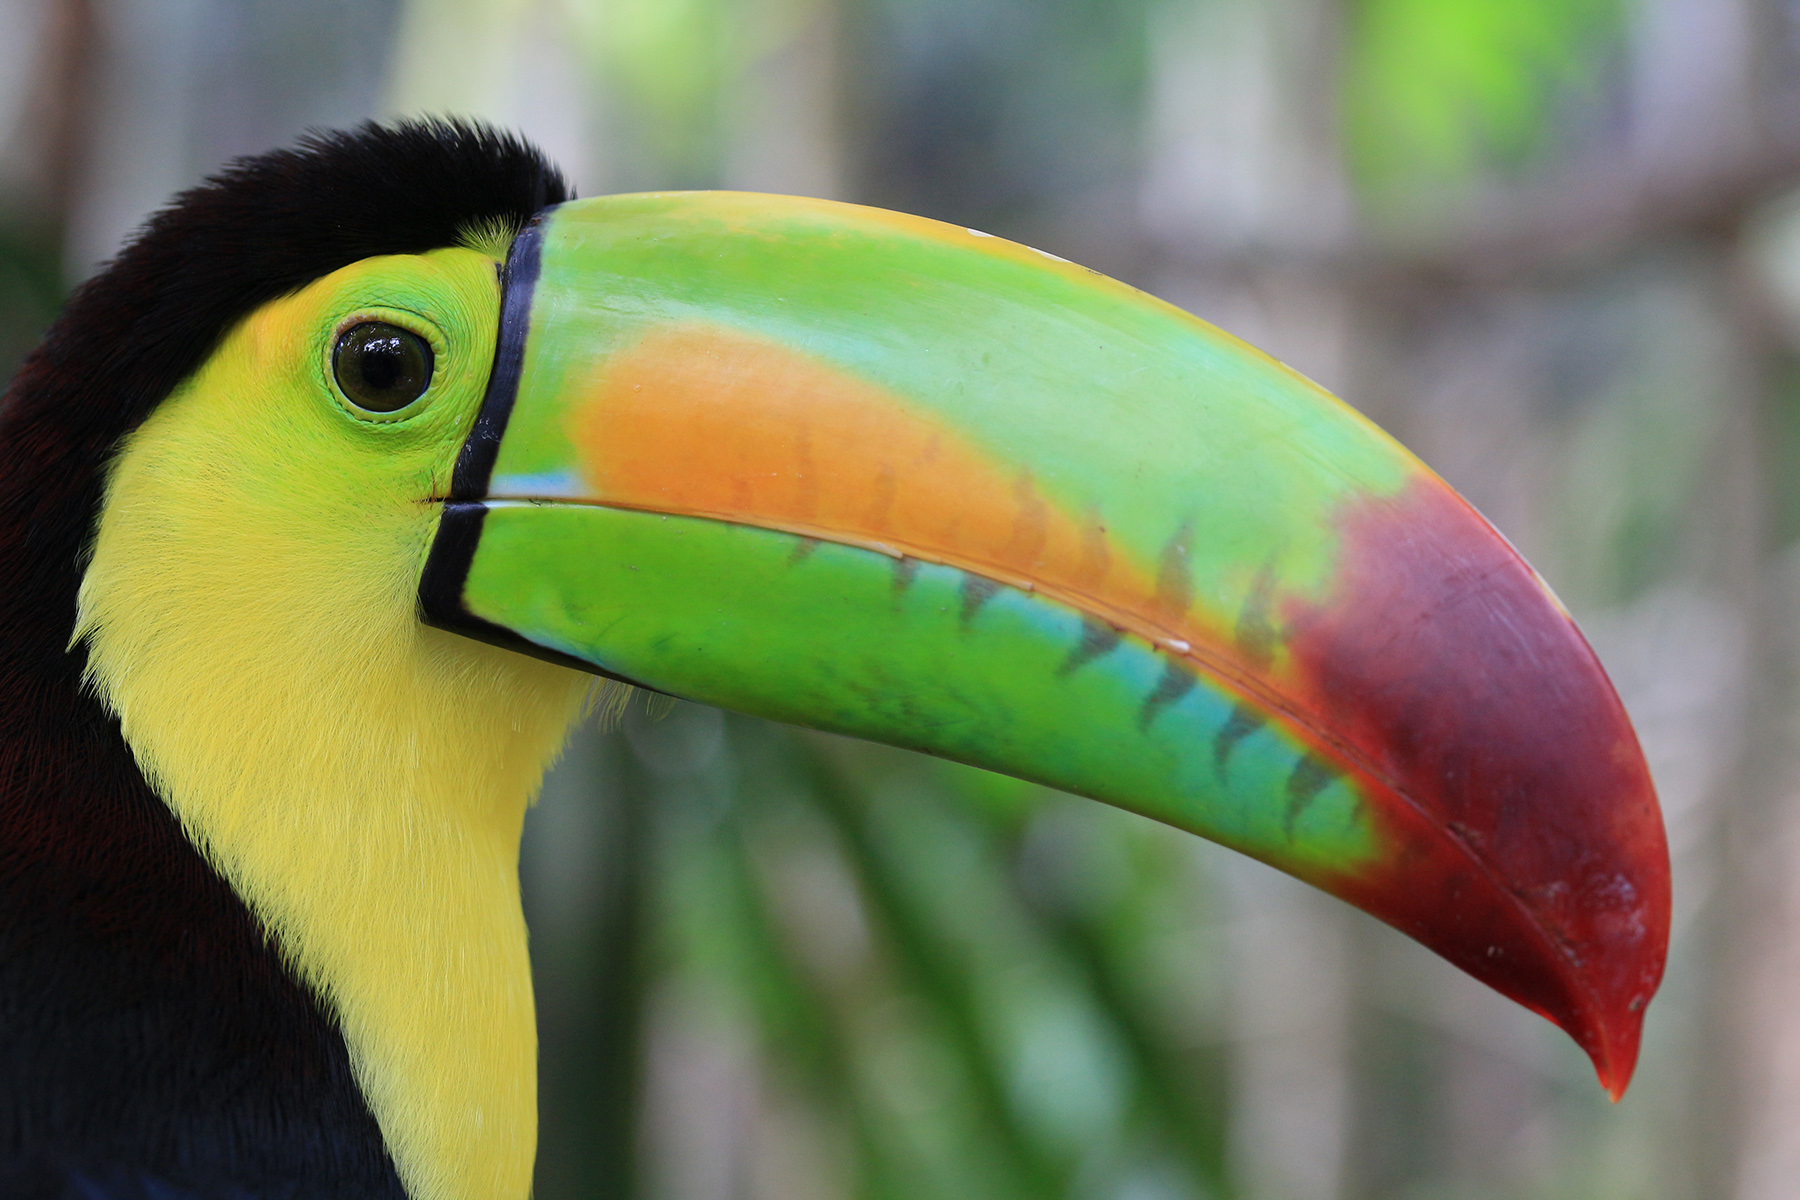
\includegraphics{sample1}
\end{frame}
%%%%%%%%%%%%%%%%%%%%%%%%%%%%%%%%%%%%%%%%%%%%%%%%%%%%%%%%%%%%%%%%%%%%%%%%%%%%%%%%%%%%%%%%%%%%%%%%%%%%%%%%%%%%%%
\begin{frame}[fragile]
\frametitle{Sub figure}
\begin{figure}
\centering
\begin{subfigure}[b]{0.3\textwidth}
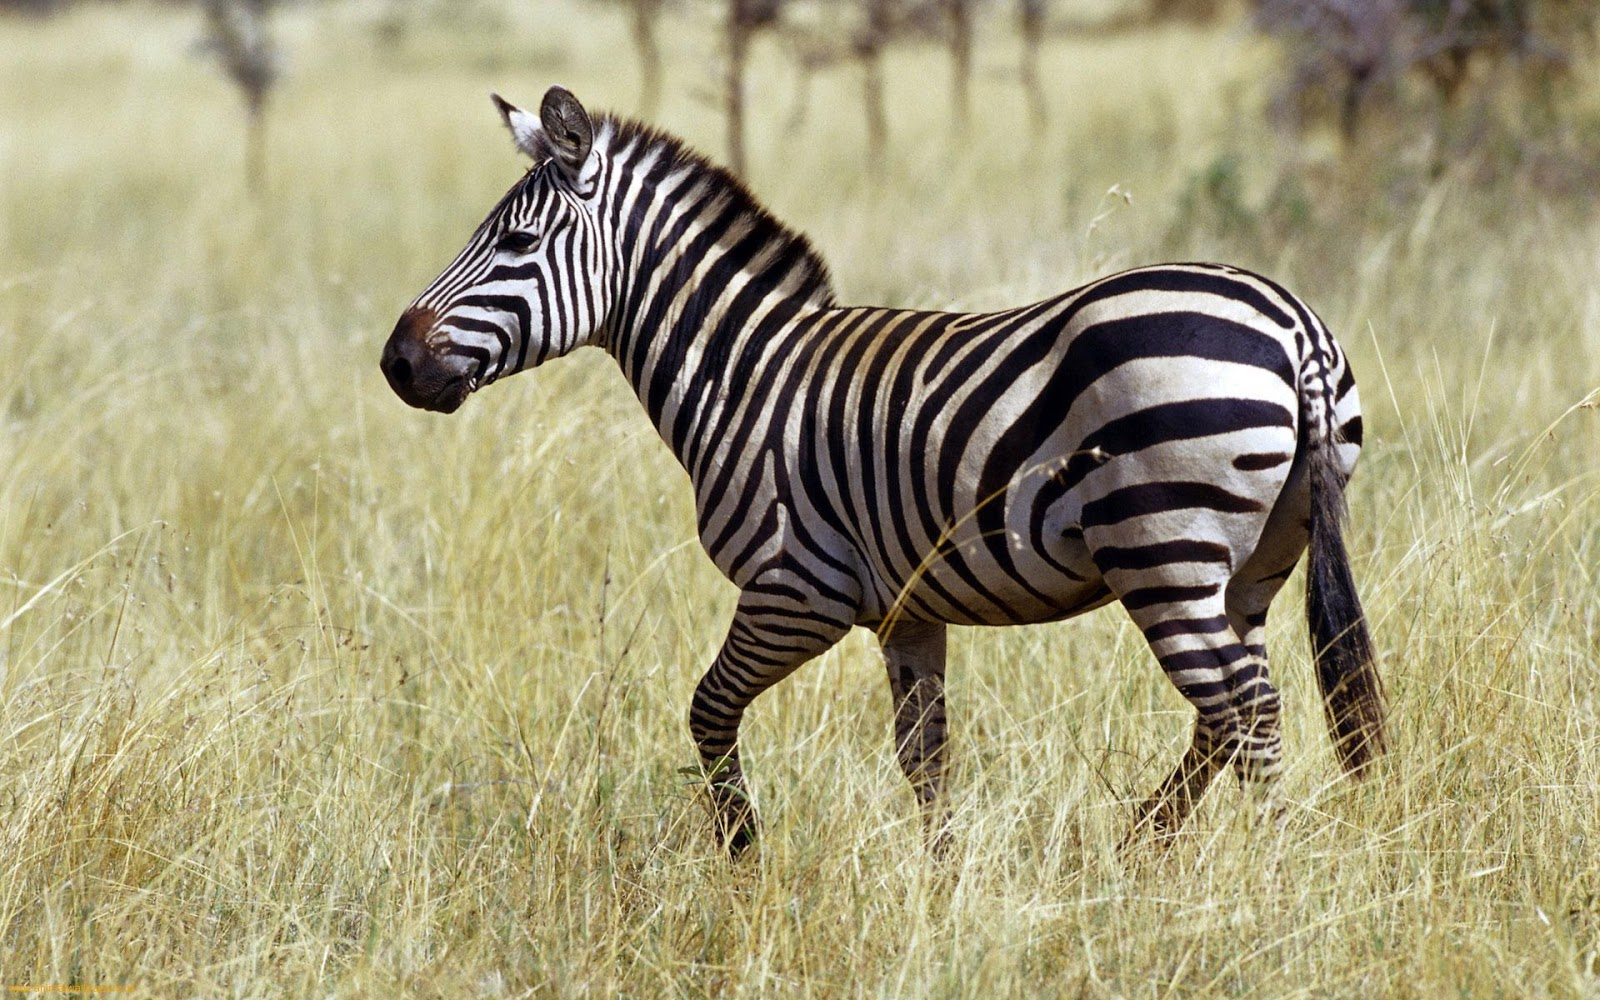
\includegraphics[width=\textwidth,height=1in]{animal1}
\caption{A Zebra}
\label{fig:Zebra}
\end{subfigure}
\begin{subfigure}[b]{0.3\textwidth}

\includegraphics[width=\textwidth,height=1in]{animal2}
\caption{A Cat}
\label{fig:cat}
\end{subfigure}
\begin{subfigure}[b]{0.3\textwidth}
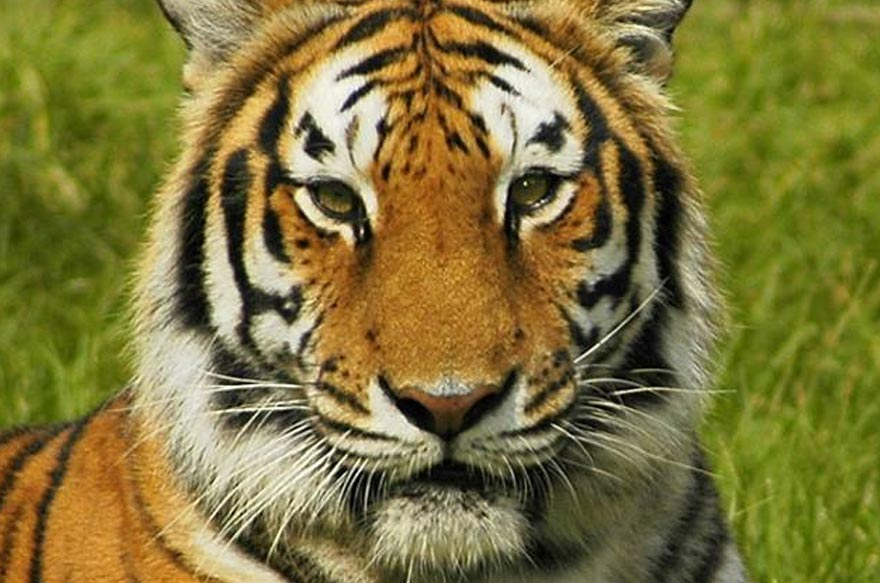
\includegraphics[width=\textwidth,height=1in]{animal3}
\caption{A Tiger}
\label{fig:tiger}
\end{subfigure}
\caption{Pictures of animals}\label{fig:animals}
\end{figure}
\end{frame}
\end{comment}
%%%%%%%%%%%%%%%%%%%%%%%%%%%%%%%%%%%%%%%%%%%%%%%%%%%%%%%%%%%%%%%%%%%%%%%%%%%%%%%%%%%%%%%%%%%%%%%%%%%%%%%%%%%%%%%%%%%%%%%%%%%%%%%%%%%%%%%%%%%%%%%%%%%%%%%%%%%%%%%%%%%%%%%%%%%%%%%%%%%%%%%%%%%%%%%%%%%%%%%%%%%%%%%%
\end{document}
